\documentclass[pointlessnumbers, abstracton, headsepline, a4paper]{scrartcl}

\usepackage[T1]{fontenc}
\usepackage[utf8]{inputenc}
\usepackage{graphicx}
\usepackage{microtype}
\usepackage{textcomp}
\usepackage{ellipsis, fixltx2e, mparhack, booktabs, longtable}
\usepackage[automark]{scrpage2}
\usepackage{multicol}
\usepackage{microtype}
\usepackage{listings}
\usepackage[a4paper]{geometry}
\usepackage[polish]{babel}

\usepackage{courier}
\lstset{
         basicstyle=\footnotesize\ttfamily, % Standardschrift
         %numbers=left,               % Ort der Zeilennummern
         numberstyle=\tiny,          % Stil der Zeilennummern
         %stepnumber=2,               % Abstand zwischen den Zeilennummern
         numbersep=5pt,              % Abstand der Nummern zum Text
         tabsize=2,                  % Groesse von Tabs
         extendedchars=true,         %
         breaklines=true,            % Zeilen werden Umgebrochen
         keywordstyle=\color{red},
         stringstyle=\color{white}\ttfamily, % Farbe der String
         showspaces=false,           % Leerzeichen anzeigen ?
         showtabs=false,             % Tabs anzeigen ?
         showstringspaces=false      % Leerzeichen in Strings anzeigen ?        
}

% part of the hyperref bundle
\usepackage{ifpdf}

\geometry{verbose,tmargin=3.5cm,bmargin=3.5cm}
\setlength{\parskip}{\medskipamount}
\setlength{\parindent}{0pt}

\clearscrheadfoot
\ohead{\\\headmark}
\ihead{
\includegraphics[scale=0.2]{img/zut2.jpg}}
\ofoot[\pagemark]{\pagemark}

% if pdflatex is used
\ifpdf

%set fonts for nicer pdf view
\IfFileExists{lmodern.sty}{\usepackage{lmodern}}
  {\usepackage[scaled=0.92]{helvet}
    \usepackage{mathptmx}
    \usepackage{courier} }
\fi

% the pages of the TOC are numbered roman
% and a pdf-bookmark for the TOC is added
\pagenumbering{arabic}
\let\myTOC\tableofcontents
\renewcommand\tableofcontents{\myTOC\clearpage\pagenumbering{arabic}}

\begin{document}
\begin{titlepage}

\begin{center}

\includegraphics[scale=0.5]{logos/zut.jpg}
\par
\end{center}

\begin{center}
\textsf{\textbf{\LARGE Wydział Informatyki}}
\end{center}{\LARGE}

\vspace{1.5cm}

\begin{center}
\textsf{\Large Metody sztucznej inteligencji}
\end{center}

\begin{center}
\textsf{\textbf{\Large Laboratorium 01 IUz-22 Urbaniak}}
\end{center}

\begin{center}
\textsf{\large Sprawozdanie}
\end{center}

\vspace{3.5cm}

\begin{center}
\begin{tabular}{ll}
Autor: & Sergiusz Urbaniak\tabularnewline
Grupa: & IUz-22\tabularnewline
Data: & \today\tabularnewline
\end{tabular}
\end{center}

\end{titlepage}

\section{Uczenie neuronu bramek logicznych}
\subsection{Bramki logicnzne}
\subsubsection{Bramka OR}

Bramka OR posiada tablice prawdy pokazaną w tablicy \ref{tab:or}.

\begin{table}[h]
\centering
\begin{tabular}[t]{c|c}
Wejście & Wyjście \\
\hline
0 0 & 0 \\
0 1 & 1 \\
1 0 & 1 \\
1 1 & 1 \\
\end{tabular}
\caption{\label{tab:or}Tablica prawdy bramki OR}
\end{table}

Wartości wejściowe są wpisane do zmiennej \texttt{we}. Dane wyjściowe według tablicy prawdy \ref{tab:or} są wpisane w zmienną \texttt{wy}. Następnie jest tworzona ``sieć'' jednego perceptronu i przeprowadzona symulacja działania sieci bez uczenia perceptronu. Kod źródłowy jest dostępny w listingu \ref{lst:or_unteached}.

\begin{center}
\begin{minipage}{0.5\textwidth}
\lstset{captionpos=b,caption=Kod nie uczonej bramki OR,label=lst:or_unteached}
\lstinputlisting{src/or_unteached.m}
\end{minipage}
\end{center}

Wykres błędu jak i danych generowany kodu \ref{lst:or_unteached} jest widoczny na rysnukach \ref{fig:or_error_unlearned} i \ref{fig:or_data_unlearned}.

\begin{figure}[h]
\centering
\begin{minipage}{0.4\textwidth}
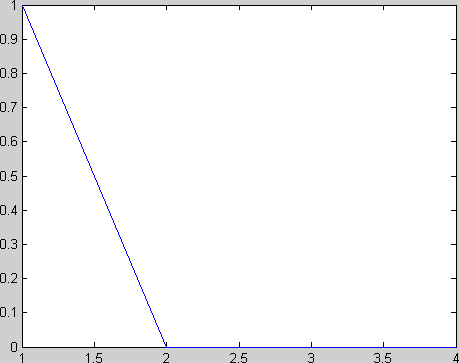
\includegraphics[scale=0.4]{figures/or_error_unlearned.png}
\caption{\label{fig:or_error_unlearned}Wykres błędu nie uczonej bramki OR}
\end{minipage}
\qquad
\begin{minipage}{0.4\textwidth}
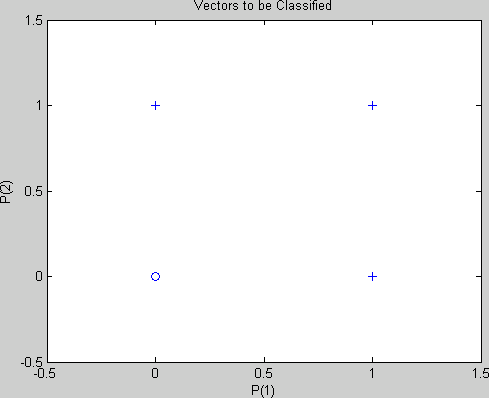
\includegraphics[scale=0.4]{figures/or_data_unlearned.png}
\caption{\label{fig:or_data_unlearned}Linia podziału danych nie uczonej bramki OR}
\end{minipage}
\end{figure}

Kod zmieniony na uczenie perceptronu jest widoczny w listingu \ref{lst:or_teached}. Dodane zostały polecenia \texttt{init} i \texttt{train}.

\begin{center}
\begin{minipage}{0.5\textwidth}
\lstset{captionpos=b,caption=Kod uczonej bramki OR,label=lst:or_teached}
\lstinputlisting{src/or_teached.m}
\end{minipage}
\end{center}

Wykres błędu jak i danych generowany kodu \ref{lst:or_teached} jest widoczny na rysnukach \ref{fig:or_error_learned} i \ref{fig:or_data_learned}. Można zaobserwowac że uczenie nie pozostawiło żadnego błędu. Perceptron poprawnie nauczył się bramki OR.

\begin{figure}[h]
\centering
\begin{minipage}{0.4\textwidth}
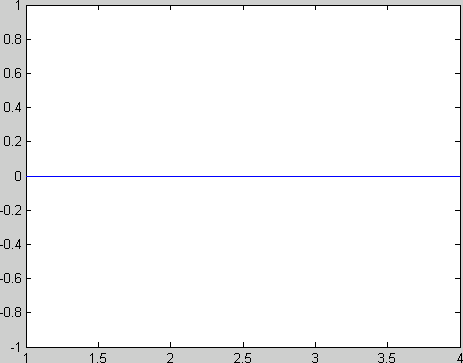
\includegraphics[scale=0.4]{figures/or_error_learned.png}
\caption{\label{fig:or_error_learned}Wykres błędu uczonej bramki OR}
\end{minipage}
\qquad
\begin{minipage}{0.4\textwidth}
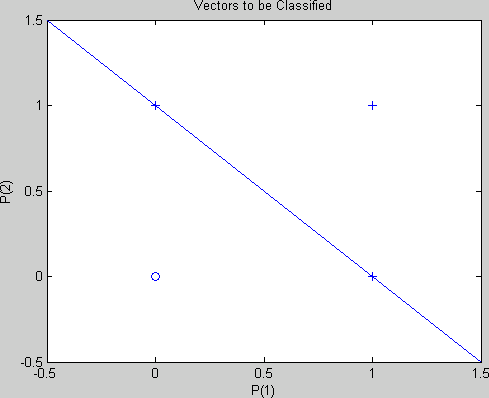
\includegraphics[scale=0.4]{figures/or_data_learned.png}
\caption{\label{fig:or_data_learned}Linia podziału danych uczonej bramki OR}
\end{minipage}
\end{figure}

\subsubsection{Bramka XOR}

Bramka XOR posiada tablice prawdy pokazaną w tablicy \ref{tab:xor}.

\begin{table}[h]
\centering
\begin{tabular}[t]{c|c}
Wejście & Wyjście \\
\hline
0 0 & 0 \\
0 1 & 1 \\
1 0 & 1 \\
1 1 & 0 \\
\end{tabular}
\caption{\label{tab:xor}Tablica prawdy bramki XOR}
\end{table}

Kod perceptronu nie uczonego jest widoczny w listingu \ref{lst:xor_unteached}. Jak widac została tylko zmieniona zmienna \texttt{wy}.

\begin{center}
\begin{minipage}{0.5\textwidth}
\lstset{captionpos=b,caption=Kod nie uczonej bramki XOR,label=lst:xor_unteached}
\lstinputlisting{src/xor_unteached.m}
\end{minipage}
\end{center}

Wykres błędu jak i danych generowany kodu \ref{lst:xor_unteached} jest widoczny na rysnukach \ref{fig:xor_error_unlearned} i \ref{fig:xor_data_unlearned}.

\begin{figure}[h]
\centering
\begin{minipage}{0.4\textwidth}
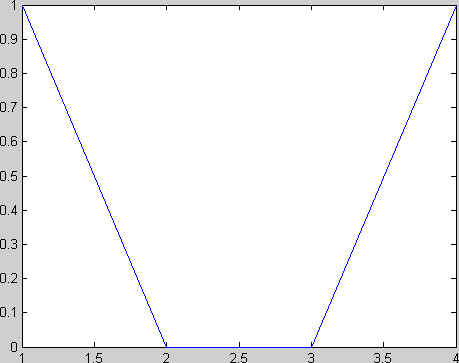
\includegraphics[scale=0.4]{figures/xor_error_unlearned.png}
        \caption{\label{fig:xor_error_unlearned}Wykres błędu nie uczonej bramki XOR}
\end{minipage}
\qquad
\begin{minipage}{0.4\textwidth}
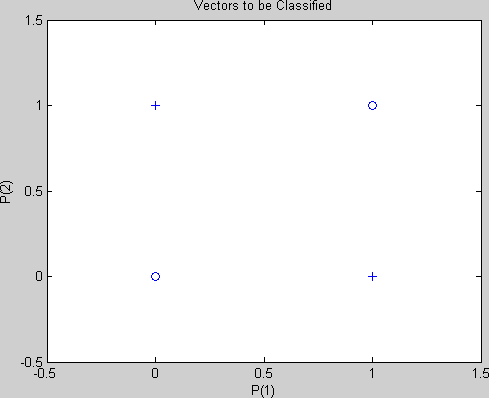
\includegraphics[scale=0.4]{figures/xor_data_unlearned.png}
\caption{\label{fig:xor_data_unlearned}Linia podziału danych nie uczonej bramki XOR}
\end{minipage}
\end{figure}

Kod zmieniony na uczenie perceptronu jest widoczny w listingu \ref{lst:xor_teached}. Znów dodane zostały polecenia \texttt{init} i \texttt{train}.

\begin{center}
\begin{minipage}{0.5\textwidth}
\lstset{captionpos=b,caption=Kod uczonej bramki XOR,label=lst:xor_teached}
\lstinputlisting{src/xor_teached.m}
\end{minipage}
\end{center}

Wykres błędu jak i danych generowany z listingu \ref{lst:xor_teached} jest widoczny na rysnukach \ref{fig:xor_error_learned} i \ref{fig:xor_data_learned}. Można zaobserwowac że uczenie nie udało się. Nadal istnieją błędy. Powodem jest fakt że podział danych bramki XOR nie jest lineowo separowalny.

\begin{figure}[h]
\centering
\begin{minipage}{0.4\textwidth}
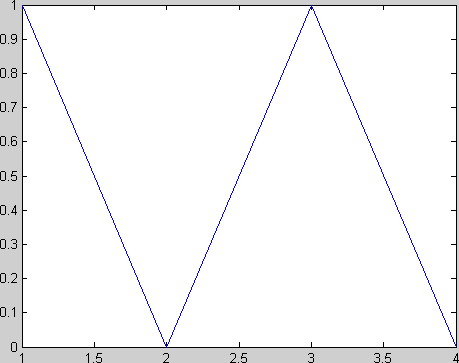
\includegraphics[scale=0.4]{figures/xor_error_learned.png}
\caption{\label{fig:xor_error_learned}Wykres błędu uczonej bramki XOR}
\end{minipage}
\qquad
\begin{minipage}{0.4\textwidth}
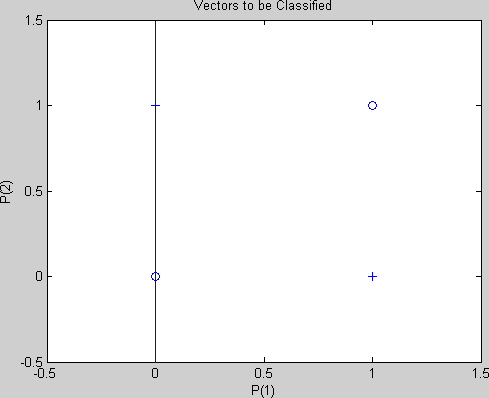
\includegraphics[scale=0.4]{figures/xor_data_learned.png}
\caption{\label{fig:xor_data_learned}Linia podziału danych uczonej bramki XOR}
\end{minipage}
\end{figure}

\subsection{Opracowanie wałsnej uczącą neuron z wzkorzystaniem reguły delta}
\subsubsection{Opis funkcji \texttt{delta}}
Zrealizowany algorytm operia się na neuronie według wzoru \ref{eq:1} i jest widoczny w listingu \ref{lst:delta.m}. Dane wejściowe $x_0, x_1, \cdots, x_n$ są wczytanę zmienną \texttt{in}.

Neuron posiada na wyjściu wartośc $y=1$ albo $y=0$ kiedy funkcja aktywacjyna $\varphi$ jest wieksza lub równa albo mniejsza od wartości $\theta$. Oczekiwane wartości wyjściowe są wczytane zmienną \texttt{out}. Uczone wartości wyjściowe są oddanę zmienną \texttt{learned}.

\begin{equation}
\label{eq:1}
\begin{array}{rcll}
y & = & \left\{
    \begin{array}{lc}
        1 & \varphi \ge \theta \\
        0 & \varphi < \theta \\
    \end{array}
\right. & \textrm{gdzie} \\
\\
\theta & = & 0 \\
\varphi & = & w_0 x_0 + w_1 x_1 + \cdots + w_n x_n + w_{n+1} b \\
b & = & 1 \\
\end{array}
\end{equation}

Wartości początkowe wag $W_0 = (w_0, w_1, \cdots , w_n)$ są wybranę przypadkowo i leżą między $[0,1]$ (linia 20 listingu \ref{lst:delta.m}). W każdej iteracji epoki uczenia są korygowane wartości wag według wzoru \ref{eq:2} (linia 55 listingu \ref{lst:delta.m}). Zmienna $0 > \eta \ge 1$ stanowi parametr uczący i jego wartośc została w tym przypadku wybrana jako $\eta = 0.2$.

$\delta$ jest różnicą między uczonymi wartościami $t$ danej epoki i wartościami wejściowymi $y$ (linia 49 listingu \ref{lst:delta.m}). Uczone dane $t$ w bierzącej epoce są wyliczane za pomocą aktualnej sumy wag i zastosowania wzoru \ref{eq:1} (linie 36-46 listingu \ref{lst:delta.m}).

\begin{equation}
\label{eq:2}
\begin{array}{rcll}
W_{i} & = & W_{i-1} + \Delta W & \textrm{gdzie} \\
\\
\Delta W & = & \eta \ \delta \ x \\
\\
\eta & = & 0.2 \\
\delta & = & t-y \\
x & = & (x_0, x_1, \cdots, x_n, b)
\end{array}
\end{equation}

Iteracyjnie wagi $W$ w każdej epoce są korygowane aż do momentu kiedy $t = y$ lub kiedy aktualna epoka jest równa maksymalnej epoce danej jako parametr \texttt{epochs} (linia 26/59 listingu \ref{lst:delta.m}).

Kod został napisany w środowisku Octave 3.0.5 pod Linux ze względu na fakt że to jest środowisko Open Source i za tym o wiele łatwej dostępne od pakietu Matlab.

\subsubsection{Kod funkcji \texttt{delta}}
\begin{center}
\lstset{numbers=left,captionpos=b,caption=\texttt{delta.m}: Funkcja ucząca neuron regułą delta,label=lst:delta.m}
\lstinputlisting{src/delta.m}
\end{center}
\end{document}

